\documentclass[../sparc.tex]{subfiles}
\graphicspath{{\subfix{../images/}}}
\begin{document}

\begin{figure}[ht]
  \centering
  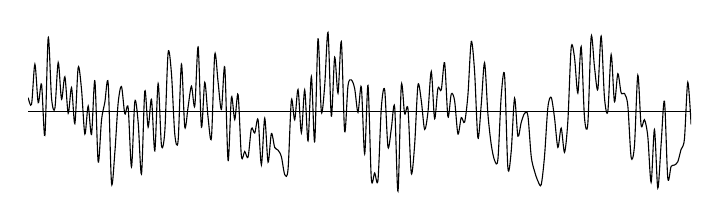
\begin{tikzpicture}[samples=200, domain=0:5*360]
    \begin{axis}[
        width=10cm, height=4cm,
        enlarge x limits=false,
        xtick=\empty,
        axis lines*=middle,
        hide y axis
      ]
      \addplot [no markers, smooth] {sin(x)+rand*2};
    \end{axis}
  \end{tikzpicture}
\end{figure}

Как правило, самая интересная часть при работе с микроконтроллерами -- это
возможность взаимодействовать с физическим миром посредством портов
ввода/вывода, располженных на отладочной плате.

В этой главе мы посмотрим, как микроконтроллер преобразует сигналы из реального
мира в цифровое представление, которое можно использовать в программе для
управления чем-либо.

\end{document}
